Suppose we have a function $f(x)$, which is continuous and differentiable over the range of interest. 
Let us also assume that we know the value $f(x_0)$ and all the derivatives at $x = x_0$. 

%.......................................
\subsubsection{First order derivatives}

The forward Taylor-series expansion for $f(x_0 + h)$, away 
from the point $x_0$ by a small amount $h$ is given by
\[
f(x_0+h)=f(x_0)+ 
h \frac{\partial f}{\partial x}(x_0)  + 
\frac{h^2}{2!} \frac{\partial^2 f}{\partial x^2}(x_0)  +
\dots  +
\frac{h^n}{n!} \frac{\partial^n f}{\partial x^n}(x_0)  
+ {\cal O}(h^{n+1})
\]
We can substract $f(x_0)$ to each side of the equation and divide by $h$:
\[
\frac{1}{h} (f(x_0+h)-f(x_0)) = 
 \frac{\partial f}{\partial x}(x_0)  + 
\frac{h}{2!} \frac{\partial^2 f}{\partial x^2}(x_0)  + \dots 
\]
and we can then express the first derivative of $f$ as follows:
\[
\frac{\partial f}{\partial x}(x_0) = \frac{f(x_0+h)-f(x_0)}{h} - 
\frac{h}{2!} \frac{\partial^2 f}{\partial x^2}(x_0) - \dots
\]
In other words, the derivative of a function $f$ at a point $x$ 
is defined by the limit:
\[
f'(x)=\lim_{h\rightarrow 0} \frac{f(x+h)-f(x)}{h}
\]


\begin{verbatim}


          --------|----------|----------|----------|---> x
                x_{i-1}     x_i       x_{i+1}


\end{verbatim}

In the context of a discrete calculation on a set of discrete points $x_i$
we can compute the first order derivative of $f$ as an approximation:
\begin{mdframed}[backgroundcolor=blue!5]
\[
\frac{\partial f}{\partial x}(x_i) = \frac{f_{i+1}-f_i}{h} + {\cal O}(h) 
\]
\end{mdframed}
where functions $f_i = f (x_i)$ are evaluated at discretely spaced $x_i$ with $x_{i+1} = x_i + h$ 
(i.e. $h=x_{i+1}-x_i$), where the node spacing, or resolution, $h$ is assumed constant.


${\cal O}(h)$ indicates that the full solution would require additional terms of order $h$, $h^2$, 
and so on. ${\cal O}$ is called the {\color{olive}truncation error}: if the distance $h$ is made smaller and smaller,
the (numerical approximation) error decreases $\propto$ $h$ in this case.

The {\bf forward FD derivative} as expressed above is called {\bf first order accurate},
and this means that very small $h$ is required for an accurate solution.
\index{general}{Forward FD Derivative}
\index{general}{Truncation Error}

We can also expand the Taylor series backward (i.e. looking 'left' of $x_0$)
\[
f(x_0-h)=f(x_0)-
h \frac{\partial f}{\partial x}(x_0)  + 
\frac{h^2}{2!} \frac{\partial^2 f}{\partial x^2}(x_0)  -
\dots 
\]
The {\bf backward FD derivative} then writes:
\[
\frac{\partial f}{\partial x}(x_i) = \frac{f_{i}-f_{i-1}}{h} + {\cal O}(h) 
\]
\index{general}{Backward FD Derivative}

Introducing the notations:
\[
f_i'=f'(x_i)=\frac{\partial f}{\partial x} (x_i)
\]




Alternatively, we can form the average of the first order accurate forward and backward schemes,
and dividing by two.
The result is the {\bf central difference} approximation,
{\bf second order accurate} of the first derivative
\[
f_i' = \frac{f_{i+1}-f_{i-1}}{2h} + {\cal O}(h^3)
\]
The denominator is $2h$ because it is the distance between point $x_{i-1}$ and $x_{i+1}$.

%.......................................
\subsubsection{Second order derivatives}

We define 
\[
f_i''=f''(x_i) = \frac{\partial^2 f}{\partial x^2} (x_i)
\]

\begin{center}
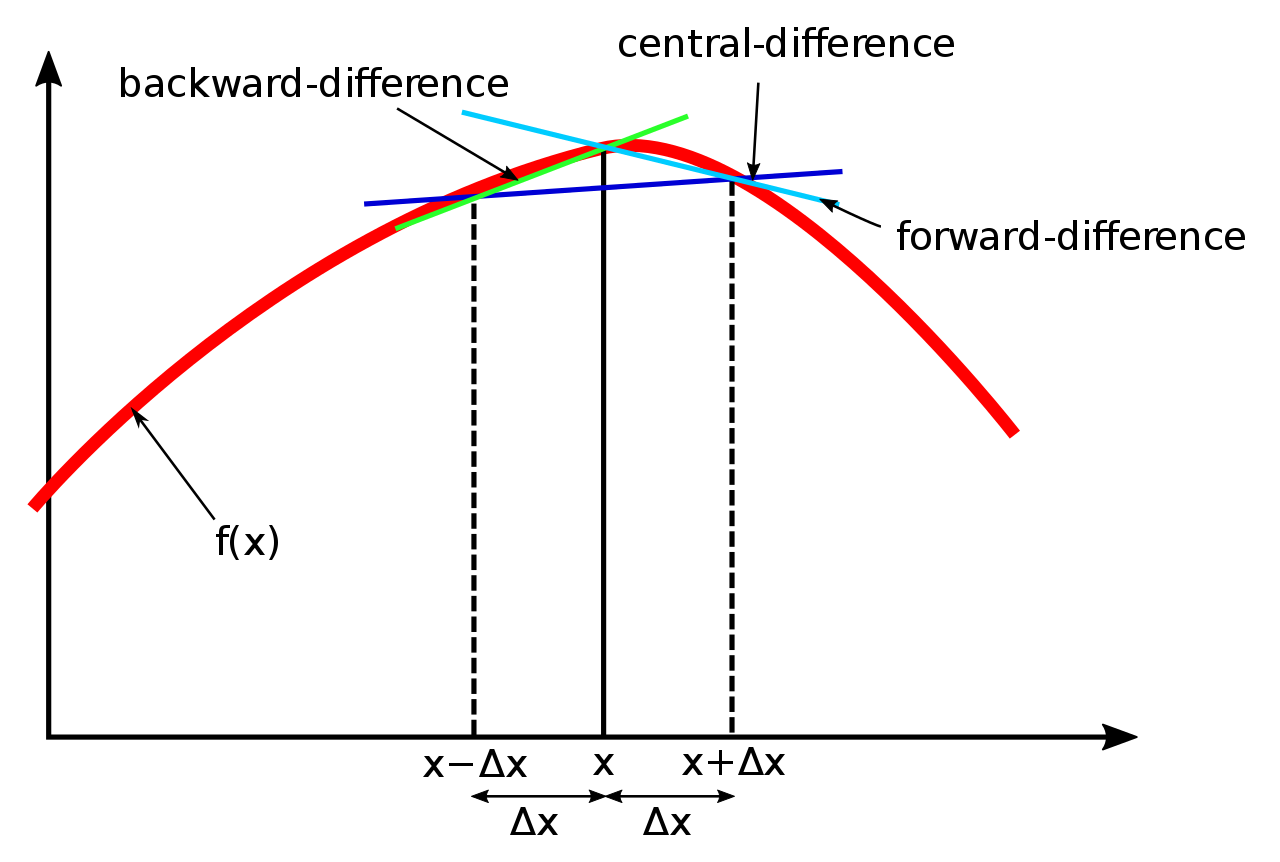
\includegraphics[width=6cm]{images/fdm/fd1}\\
Stolen from wikipedia - REDO
\end{center}


%______________________________
\paragraph{Second order forward}. 

Let us define $g=f'$. Then 
\[
g_i' = \frac{g_{i+1}-g_{i}}{h}
\]
On the one hand, we have $g_i'=g'(x_i)=f''(x_i)=f_i''$ and on the other hand
\[
g_i' = \frac{f_{i+1}'-f_{i}'}{h}
\]
so we can use the forward derivative formula twice for $f_{i+1}'$ and $f_{i}'$ and 
obtain the following second order derivatives of $f$:
\[
f_{i}'' 
= \frac{f_{i+1}'-f_i'}{h} 
%+ {\cal O}(h^2)
= \frac{\frac{f_{i+2}-f_{i+1}}{h}-
\frac{f_{i+1}-f_i}{h}
}{h} 
%+ {\cal O}(h^2)
= \frac{f_{i+2}-2f_{i+1}+f_i}{h^2} 
%+ {\cal O}(h^2)
\]
which is the {\bf first order accurate}, {\bf forward difference} approximation for
second order derivatives at $x_{i}$.

%______________________________
\paragraph{Second order backward}. 

Likewise, we obtain the following formula when using the backward derivative twice:

\[
f_{i}'' 
= \frac{f_{i}'-f_{i-1}'}{h} 
%+ {\cal O}(h^2)
= \frac{\frac{f_{i}-f_{i-1}}{h}- \frac{f_{i-2}-f_{i-1}}{h}  }{h} 
%+ {\cal O}(h^2)
= \frac{f_{i}-2f_{i-1}+f_{i-2}}{h^2} 
%+ {\cal O}(h^2)
\]





%______________________________
\paragraph{Second order central} 
By adding the taylor expansions (with $+h$ and $-h$) 
a {\bf second order accurate}  approximation of the second derivative is obtained.
We start from 

\[
f(x_0+h)=f(x_0)+ 
h \frac{\partial f}{\partial x}(x_0)  + 
\frac{h^2}{2!} \frac{\partial^2 f}{\partial x^2}(x_0)  +
\dots  +
\frac{h^n}{n!} \frac{\partial^n f}{\partial x^n}(x_0)  
+ {\cal O}(h^{n+1})
\]
\[
f(x_0-h)=f(x_0)+ 
-h \frac{\partial f}{\partial x}(x_0)  + 
\frac{h^2}{2!} \frac{\partial^2 f}{\partial x^2}(x_0)  +
\dots  +
\frac{h^n}{n!} \frac{\partial^n f}{\partial x^n}(x_0)  
+ {\cal O}(h^{n+1})
\]
and we see that adding the first equation to the second yields

\[
f(x_0+h) + f(x_0-h) =2 f(x_0)+ 
\underbrace{h \frac{\partial f}{\partial x}(x_0)   
-h \frac{\partial f}{\partial x}(x_0)}_{=0}  + 
\frac{h^2}{2!} \frac{\partial^2 f}{\partial x^2}(x_0)  +
\frac{h^2}{2!} \frac{\partial^2 f}{\partial x^2}(x_0)  +
\dots  +
\frac{h^n}{n!} \frac{\partial^n f}{\partial x^n}(x_0)  
+ {\cal O}(h^{n+1})
\]
or, 
\[
\frac{\partial^2 f}{\partial x^2}(x_0)  =
\frac{f(x_0+h) -2f(x_0) + f(x_0-h) }{h^2}
+ {\cal O}(h)
\] 
which translates into
\[
f_{i}''=\frac{f_{i+1}-2f_i+f_{i-1}}{h^2} 
\]


\begin{verbatim}

                         x_{i-1/2)           x_{i+1/2}
          --------|----------+----------|---------+----------|-------------> x
                x_{i-1}                x_i                x_{i+1}


\end{verbatim}
Another way to arrive at the same expression is to write the expansion at $x_0 \pm h/2$, 
i.e. at the (convenient yet inexistant) half points $i\pm 1/2$:
\[
f_{i+1/2}'=\frac{f_{i+1}-f_i}{h}
\quad\quad
\quad\quad
f_{i-1/2}'=\frac{f_{i}-f_{i-1}}{h}
\]
\begin{mdframed}[backgroundcolor=blue!5]
\[
f_i''=\frac{f_{i+1/2}'-f_{i-1/2}'}{h} = 
\frac{f_{i+1}-2f_i+f_{i-1}}{h^2} 
\]
\end{mdframed}
Note that derivatives of the form (see Heat Transport Equation) 
\[
\frac{\partial }{\partial x} \left(  k  \frac{\partial f}{\partial x} \right)
\]
where $k$ is a function of space, should be formed as follows
\[
\left. \frac{\partial }{\partial x} \left(  k  \frac{\partial f}{\partial x} \right) \right|_i
=
\frac{ k_{i+1/2} \frac{f_{i+1}-f_i}{h} - k_{i-1/2}\frac{f_i-f_{i-1}}{h}    }{h} + {\cal O}(h^3)
\]
where $k_{i\pm 1/2}$ is evaluated between the points to maintain the second order accuracy.

{\tiny
Note: If $k$ has strong jumps from one grid point to another that are not aligned with
the grid-nodes, most second-order methods will show first order accuracy at best.}
















